\chapter{Market Analysis}\label{ch:C}
\section{Competitive Analysis}\label{companl}
Nowadays, more and more students are looking for platforms that will help them share knowledge and skills, especially students who need help with examples in documentation code, and so on. Online resources such as headhunter.kz \cite{headhunter}, Stackoverflow.com \cite{stackoverlow}, Reddit.com \cite{reddit}.
They offer a wide range of job search, ask questions, answer them, and so on, which allows students to study effectively. However, there is a need for specialized platforms for university students, where they could share knowledge and support joint projects within the university in order to be more effective.The increasing interest in crowdfunding also points to the need to create a platform that will bring students together to implement their projects with the help of community support or investors. Thus, the market has the potential to develop an innovative platform that will connect university students and provide them with opportunities to share knowledge, support projects and attract funding through crowdfunding \cite{crowdfunding}, as well as ask questions by answering them, that is, create one large community.

\begin{figure}[ht]\label{fig:market}
  \centering
  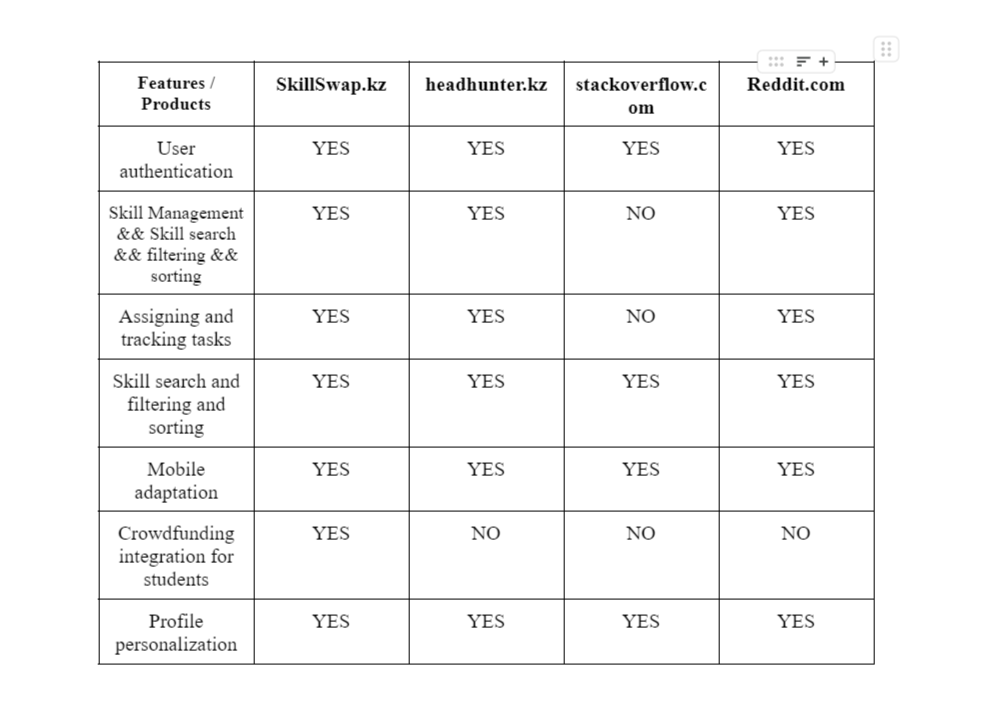
\includegraphics[width=0.75\linewidth]{figures/market analyse.png}
  \caption{Market analyse.}
\end{figure}
\newpage
\section{Product Analysis}\label{prdanl}
\subsection{Target Audience}\label{trganl}

The target audience for this product according to our questionnaire, all screenshots of the questions will be provided at the end of the document this target audience from our survey \cite{survey}:
\par
Gender: Men (87.5 in percent) and Women (12.5 in percent) 
\par
Age: 16 - 18 (7.7 in percent), 19 - 21 (69.21 in percent), 22 - 25 (23.1 in percent)
\par
Status: Students (100 in percent)
\par
Location: Kazakhstan
\subsection{Target Market}\label{trgmrk}
The type of application that will work for our users is the B2C domain. It turns out that this will be a kind of freelance among students; self-freelance means that these are self-employment specialists who will provide their services to others for money or for free, and this scheme will work in our web application and on the phone. Determine our target market area. 
\par
We used method \href{https://www.insales.ru/blogs/university/metodika-5w-marka-sherringtona}{5 W} on that:
\par
\begin{itemize}
    \item \textit{What - What are you selling ?}
    \par
    Online platform where can students get skills which their prefer.
    \item \textit{Who - Who buys your products?}
    \par
    All students from Kazakhstan.
    \item \textit{Where — Where do you sell?}
\par Our web platform and mobile.
    \item \textit{When — When does a customer have a need for a product?}
\par When they want to get skills from another person and maybe they will be friends.
    \item \textit{Why — Why should the customer buy the product from you?}
    \par
    Basically it's gonna be a free but to get new futures and able to do donate for another person to give motivation to do the best projects in the world.
\end{itemize}